
\chapter{Introduction}
\label{chap:introduction}

Since the cessation of full-scale nuclear testing, numerical simulation has become a central tool for the study and maintenance of nuclear deterrence capabilities. In this context, understanding high-energy-density physics phenomena is of major importance. These regimes involve extreme thermodynamic conditions, strong compressibility effects, shock waves, radiation transport, and hydrodynamic instabilities. Since such conditions cannot be fully reproduced using conventional laboratory experiments, dedicated experimental platforms and high-fidelity numerical simulations are required to investigate them.

Among these experimental platforms, Inertial Confinement Fusion (ICF) provides a privileged framework for studying matter under extreme pressure and temperature conditions. In ICF, a small capsule containing deuterium--tritium fuel is rapidly compressed by high-intensity laser beams. The ablation of the capsule outer layer generates an inward pressure, leading to the compression and heating of the fuel. If the implosion is sufficiently symmetric and efficient, thermonuclear reactions may occur before the target disassembles.

\begin{figure}[h]
\centering

\includegraphics[width=0.40\textwidth]{figures/intro/fci.png}
\caption{Schematic representation of an inertial confinement fusion target and laser-driven implosion process.}
\label{fig:icf_principle}
\end{figure}

A major difficulty in ICF lies in maintaining the stability of the implosion. Small perturbations initially present at material interfaces may grow during the acceleration phase and progressively degrade the compression quality. Among the hydrodynamic instabilities involved in this process, the Rayleigh--Taylor instability plays a central role. It occurs when a dense fluid is accelerated by a lighter one and leads to the development of characteristic bubble and spike structures. In the context of ICF, this instability may enhance turbulent mixing between the shell material and the fuel, thereby reducing the achievable temperature and compromising ignition conditions.

Predicting the evolution of the Rayleigh--Taylor instability remains challenging because of its non-linear, multi-scale, and eventually turbulent nature. Direct Numerical Simulations (DNS) provide a reference approach to study such flows, as they resolve the relevant spatial and temporal scales without relying on turbulence closure models. They therefore make it possible to generate accurate representations of the instability dynamics, from the early growth phase to more complex mixing regimes.

However, DNS are extremely expensive from a computational point of view. Their cost increases rapidly with the spatial resolution, the duration of the simulation, and the complexity of the physical model. As a consequence, only a limited number of simulations can generally be produced, which strongly constrains the size of the available datasets. This limitation is particularly important when considering data-driven approaches, whose performance often depends on the quantity and diversity of training data.

\begin{figure}[h]
\centering
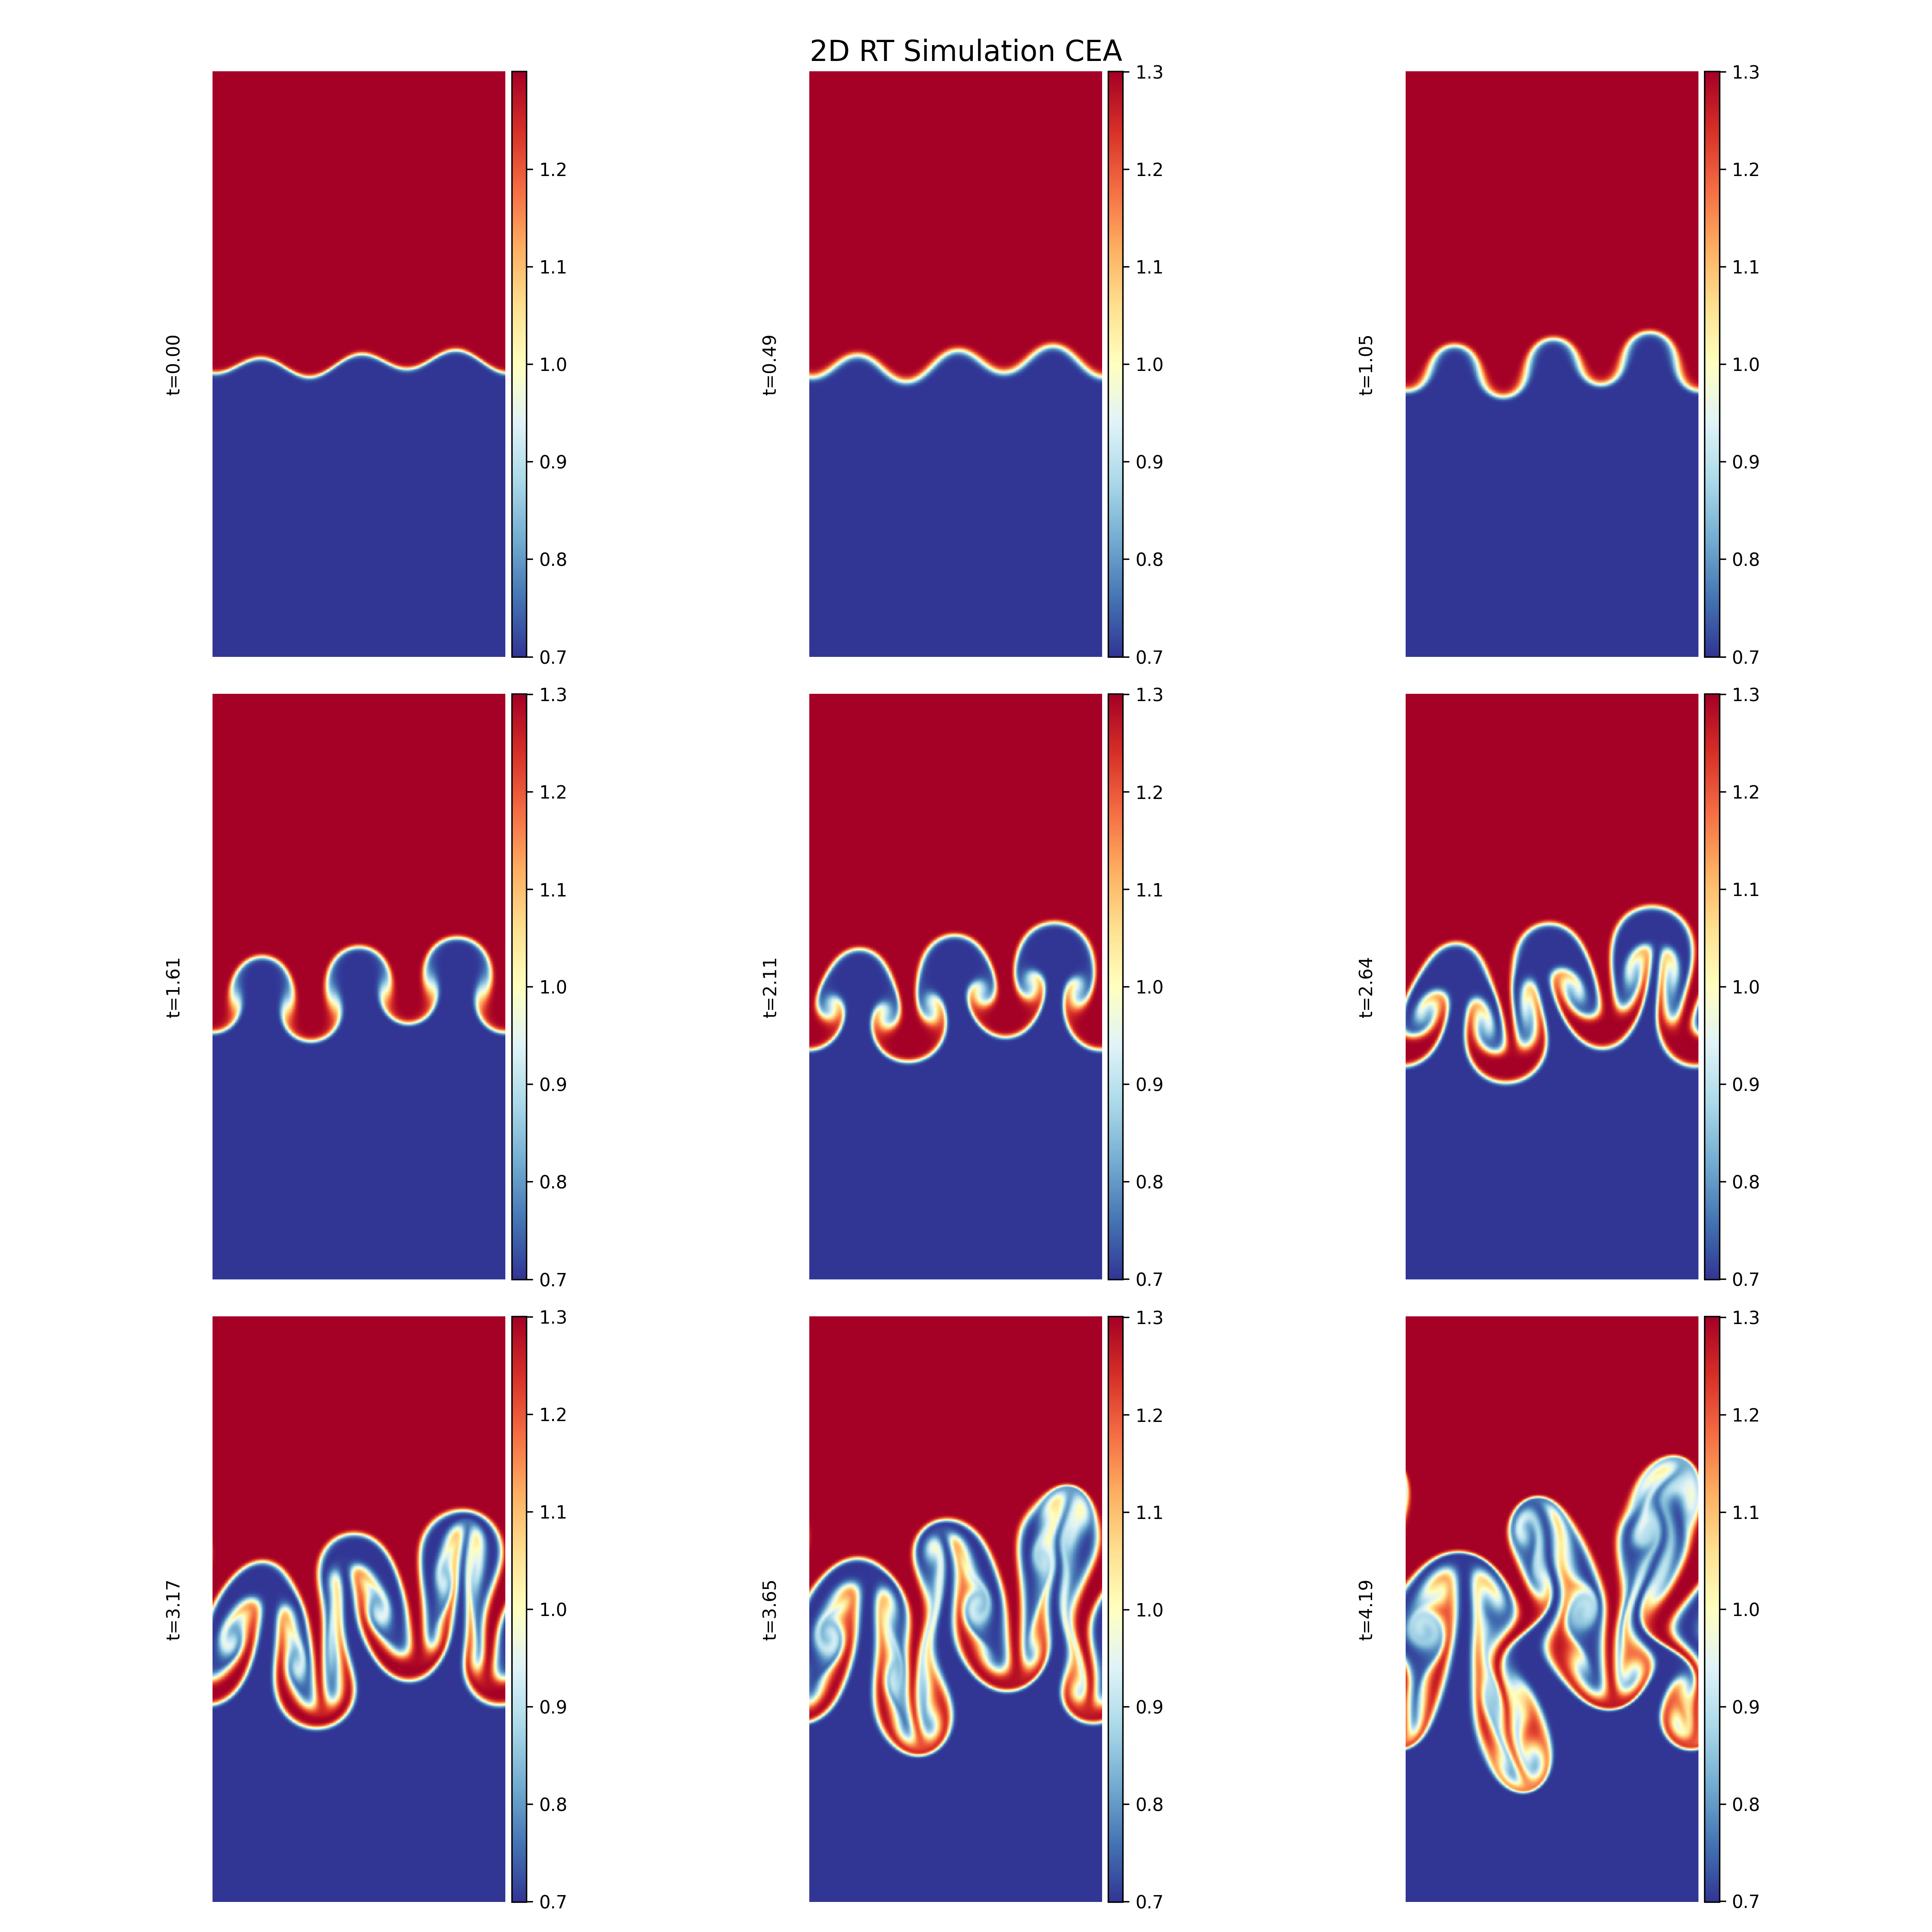
\includegraphics[width=0.8\textwidth]{figures/intro/RTCEA_simulation_2D.png}
\caption{Example of density field evolution obtained from Direct Numerical Simulations of the Rayleigh--Taylor instability}
\label{fig:dns_example}
\end{figure}

This context motivates the development of surrogate models able to reproduce, at a reduced computational cost, the statistical properties of fields generated by high-fidelity simulations. In recent years, machine learning methods have become increasingly attractive for this purpose. In particular, generative models aim to learn a probability distribution from a set of reference examples, so that new samples can be drawn from the same underlying distribution. In the present case, this distribution is intended to represent the ensemble of possible density fields produced by the numerical simulations. Diffusion models constitute a promising class of generative models for this task, as they are designed to learn complex high-dimensional probability distributions.

The objective of this master thesis is to investigate the use of diffusion-based generative models for two-dimensional Rayleigh--Taylor instability fields obtained from DNS. More specifically, the goal is to approximate the probability distribution of the simulated density fields and to evaluate whether generated samples can reproduce the main visual and statistical features of the reference data. Because the available dataset is limited, particular attention is given to multi-scale representations.

Wavelet decompositions provide a framework for this purpose. They represent a field through components associated with different spatial scales and locations, separating coarse structures from finer details. This property is well suited to Rayleigh--Taylor flows, where large-scale interface deformation and small-scale mixing structures coexist. Introducing a wavelet decomposition before the diffusion model may therefore help the generative process focus on scale-dependent features of the flow and make better use of the limited training data.

\begin{figure}[H]
\centering
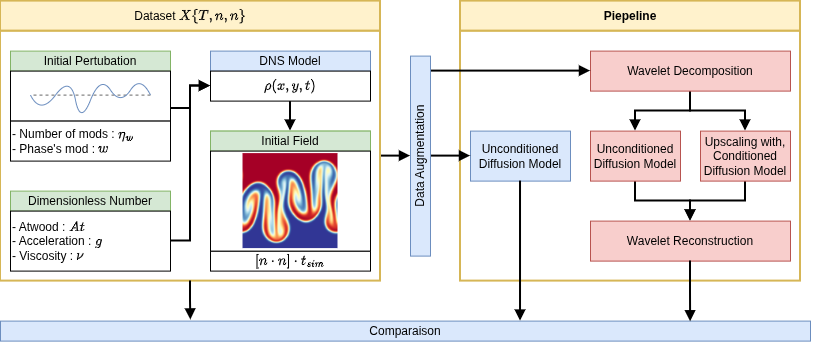
\includegraphics[width=0.8\textwidth]{figures/intro/pipeline.png}
\caption{General principle of the diffusion-based surrogate modeling approach used in this work}
\label{fig:introduction_diffusion_pipeline}
\end{figure}

The work presented in this report follows two main directions. First, a classical diffusion model is implemented and trained directly on preprocessed Rayleigh--Taylor density fields, providing a baseline generative approach. Second, a wavelet-based diffusion strategy is investigated in order to assess whether a multi-resolution representation can improve the quality, stability, or data efficiency of the generation process. The comparison between these two approaches constitutes the central objective of this study.


\section{Project Objectives and Contributions}

The internship objective is to design and evaluate generative surrogate models for two-dimensional Rayleigh--Taylor instability fields. The main contributions of this work are:
\begin{itemize}
\item the implementation of a baseline diffusion model trained directly on preprocessed density fields;
\item the construction of physically consistent data augmentation strategies adapted to the symmetries and periodicity of the dataset;
\item the study of Fourier and wavelet representations as tools for dimensionality reduction and multi-scale analysis;
\item the design of a wavelet-based diffusion pipeline intended to exploit the scale-separated structure of RTI fields;
\item the definition and use of evaluation metrics combining feature-space distances and physical statistical indicators.
\end{itemize}


\section{Report Outline}

Chapter~\ref{chap:related-work} positions the project with respect to existing scientific and machine-learning approaches. Chapter~\ref{chap:background} introduces the physical, numerical, and mathematical background required to understand the work. Chapter~\ref{chap:methodology} details the implemented methodology. Chapter~\ref{chap:experiments} presents the dataset, experiments, metrics, and results. Chapter~\ref{chap:conclusion} summarizes the work and discusses limitations and perspectives.

